\chapter{RESULTS}
\label{chp:results}

In addition to employing grid search and built-in cross-validation to optimize the classifiers described in Chapter \ref{chp:methods}, the impact of two methods to rescale the features was evaluated: normalization and standardization. Further more, the influence of \gls{pca} by considering 98\% of the explained variance was also investigated, resulting in approximately a 50\% reduction in the number of features. The results were evaluated in Excel, with examples using the ESC-10 dataset depicted in Figures \ref{fig:results_ESC-10_classification_results_overview} and \ref{fig:results_ESC-10_classification_results_fold_overview}. The results are compiled in the subsequent sections only as tables.

\begin{figure}[htbp]
    \raggedright
        \caption{Overview of the classifiers results during the training / classification flow - Example with the ESC-10 dataset.}
        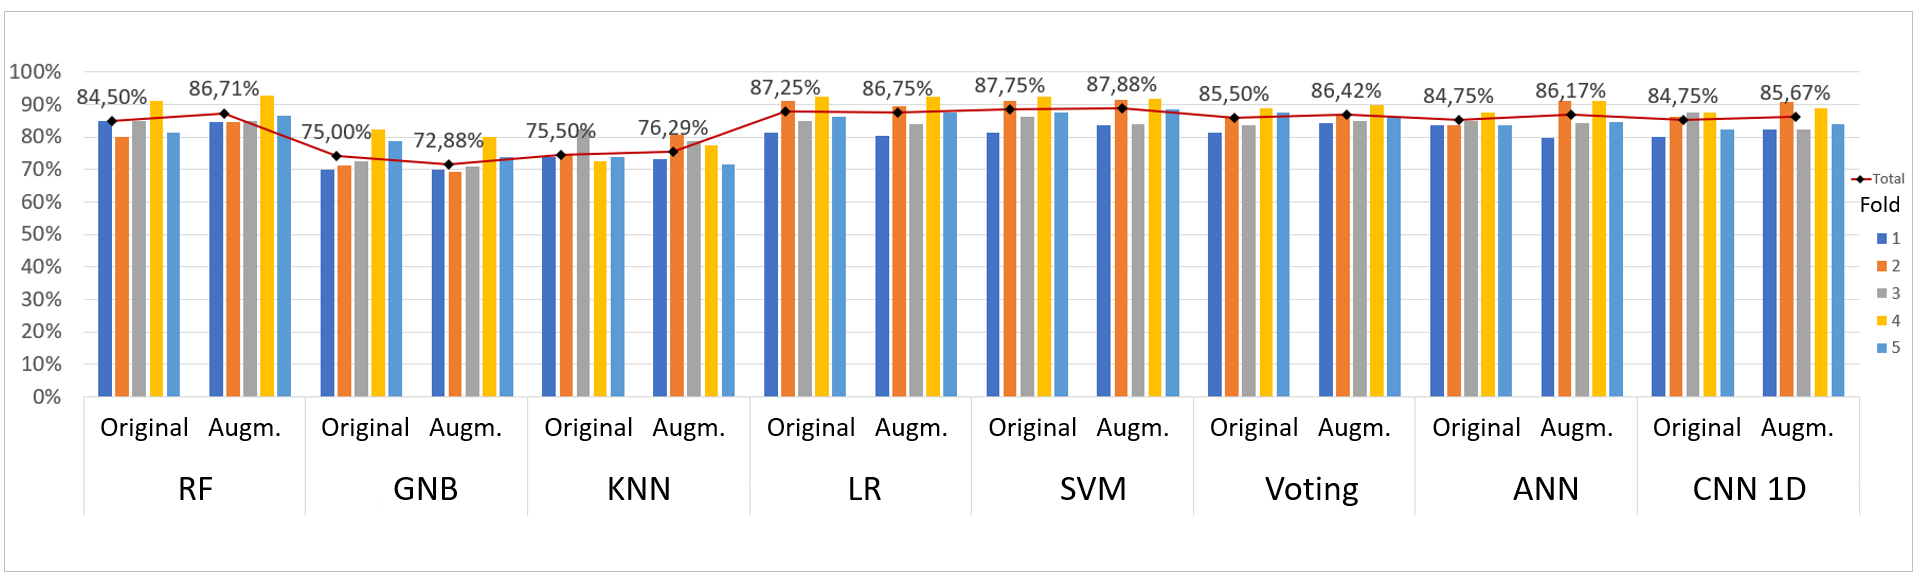
\includegraphics[width=1\textwidth]{resources/images/060-results/Results_classification_flow_ESC-10_1.png}
        \smallcaption{Source: Author}
        \label{fig:results_ESC-10_classification_results_overview}
\end{figure}

\begin{figure}[htbp]
    \raggedright
        \caption{Comparison of the best option for the classifiers results per fold during the training / classification flow - Example with the ESC-10 dataset standardized x standardized + PCA}
        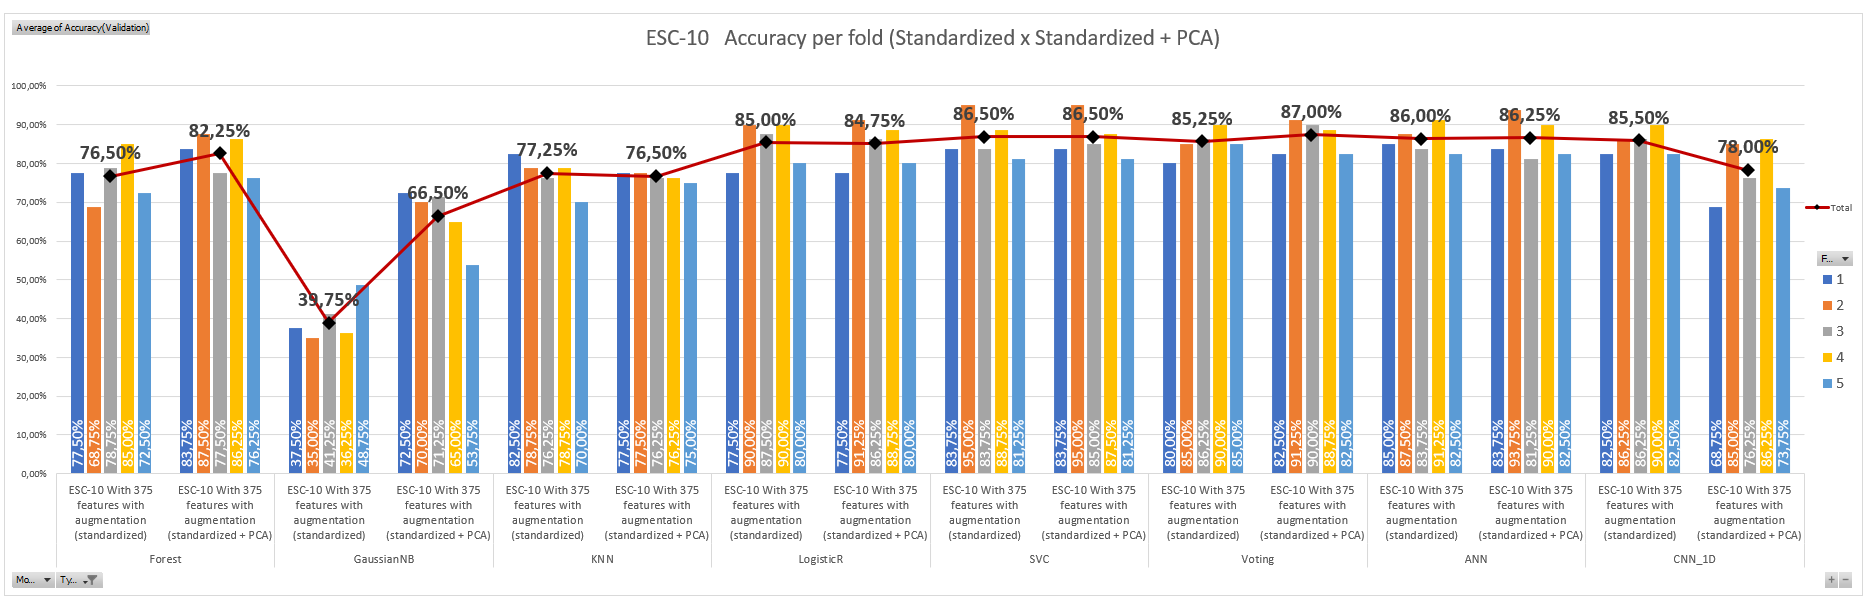
\includegraphics[width=1\textwidth]{resources/images/060-results/Results_classification_flow_ESC-10_2.png}
        \smallcaption{Source: Author}
        \label{fig:results_ESC-10_classification_results_fold_overview}
\end{figure}


\section{BENCHMARK}
\label{sec:results_metrics}

% Specific objective a) 

This section presents the basic benchmark metrics gathered within the body of literature (Chapter \ref{chp:rel}). Starting with human accuracy, according to \textcite{PiczakESC2015} an average accuracy rate of 95,7\% was attained for the ESC-10 dataset, while the ESC-50 dataset achieved an accuracy rate of 81,3\%. The recall rates for individual sound event classes displayed significant variation, ranging from 34,1\% for washing machine noise to nearly 100\% for crying babies and barking dogs. These experiments indicate that proficient and attentive listeners have the potential to achieve perfect scores on the smaller dataset and are likely to reach accuracy levels of approximately 90\% on the main dataset, albeit with some uncertainties when categorizing more ambiguous mechanical noises and soundscapes.

To ensure the soundness of the \gls{esr} algorithm, accuracy rates of benchmark datasets were initially compiled from the literature, but only the ones that fully comply with the dataset specifications, more specifically, with k-fold cross-validation setting of 5 for ESC-10, 3 for BDLib2 and 10 for \gls{us8k}. Thus the values were collected from \textcite{PiczakESC2015}, \textcite{Bountourakis2019}\footnote{The \gls{eti} method achieved higher results, with 81,5\% \gls{ann}, 80,4\% \gls{glm}, and 74,8\% \gls{lr}.} with \gls{sti} method,  \textcite{Salamon2014}, and \textcite{Vandendriessche2021} in the Table \ref{table:results_benchmark_accuracy}.

\begin{table}[ht!]
    \caption[Accuracy results benchmark of the datasets]{Compilation of the accuracy results to establish a benchmark on the utilized datasets.}
    \label{table:results_benchmark_accuracy}
    \centering
    \begin{tabular}{
        >{\centering\arraybackslash}m{0.28\textwidth} | >
        {\centering\arraybackslash}m{0.20\textwidth} | >
        {\centering\arraybackslash}m{0.20\textwidth} | >
        {\centering\arraybackslash}m{0.20\textwidth}}
        \Xhline{2\arrayrulewidth}
        \rowcolor{lightgray}
        \textbf{Classifier} & \textbf{ESC-10} & \textbf{BDLib2} & \textbf{\gls{us8k}}\\
        \hline
        \gls{k-nn} & 66,7\% & --- & 56,0\%\\
        \hline
        \gls{gnb}  & --- & --- & --- \\
        \hline
        \gls{svm} &  67,0\% & --- & 69,0\%   \\
        \hline
        \gls{lr} & --- & 73,6\% & --- \\
        \hline
        Random Forest & 72,7\% & --- & 66,0\% \\
        \hline
        Voting soft & --- & --- & 10,0\%  \\
        \hline
        \gls{ann} & --- & 75,2\% & ---  \\
        \hline
        \gls{cnn} 1D & 83,2\% & 74,4\% & 60,1\%  \\
        \hline
        \gls{glm} & --- & 75,0\% & ---  \\
        \hline
        Decision tree & --- & --- & 48,0\%  \\
        \hline
        \gls{cnn} 2D & ??? & ??? & ???  \\
     \Xhline{2\arrayrulewidth}
    \end{tabular}
    \smallcaption{Source: Author}
\end{table}

\section{TRAINING AND CLASSIFICATION FLOW}
\label{sec:results_training_classification_flow}

In this initial stage of the experiments, the main objective is to evaluate the \gls{esr} algorithm implemented in several classifiers regarding its feature selection, feature extraction, classification metrics, processing memory, allocation memory and response time. The evaluation was performed both in a notebook environment and embedded in the Raspberry Pi 4.

To evaluate feature selection, a Python script was developed to generate various models for k-fold cross-validation. These models included normalization, standardization, normalization + \gls{pca}, and standardization + \gls{pca}. Each model was applied to both the original and augmented datasets. On average, the accuracy rates of the top-performing classifiers increased among the datasets: 4,7\% in the  ESC-10, 11,3\% in the BDLib2, and 1,7\% in the \gls{us8k}. It could also be observed that the \gls{us8k} dataset was the least impacted by the augmentation, which is understandable considering its substantial total duration of 8,75 hours (8.732 samples), in contrast to the 0,55 hours (400 samples) of the ESC-10 and 0,5 hours (180 samples) of the BDLib2 datasets. Notably, Random Forest was less affected while the neural networks, \gls{ann} and \gls{cnn} 1D, benefited the most from the augmentation. Further more, as depicted in Table \ref{table:results_accuracy_overview_classifiers_aug_ori_1}, the winning classifiers were mostly the models \textbf{augmented standardized} and \textbf{augmented standardized + \gls{pca}}. The differences between the exceptions and these models were marginal.

\begin{table}[ht!]
    \caption[Accuracy rates overview using the benchmark datasets - Models augmented x original (Focus on the classifiers line by line)]{Accuracy rates overview using the benchmark datasets - The color gradient is focused on the classifiers utilized in the models augmented and original, line by line.}
    \label{table:results_accuracy_overview_classifiers_aug_ori_1}
     \raggedright
    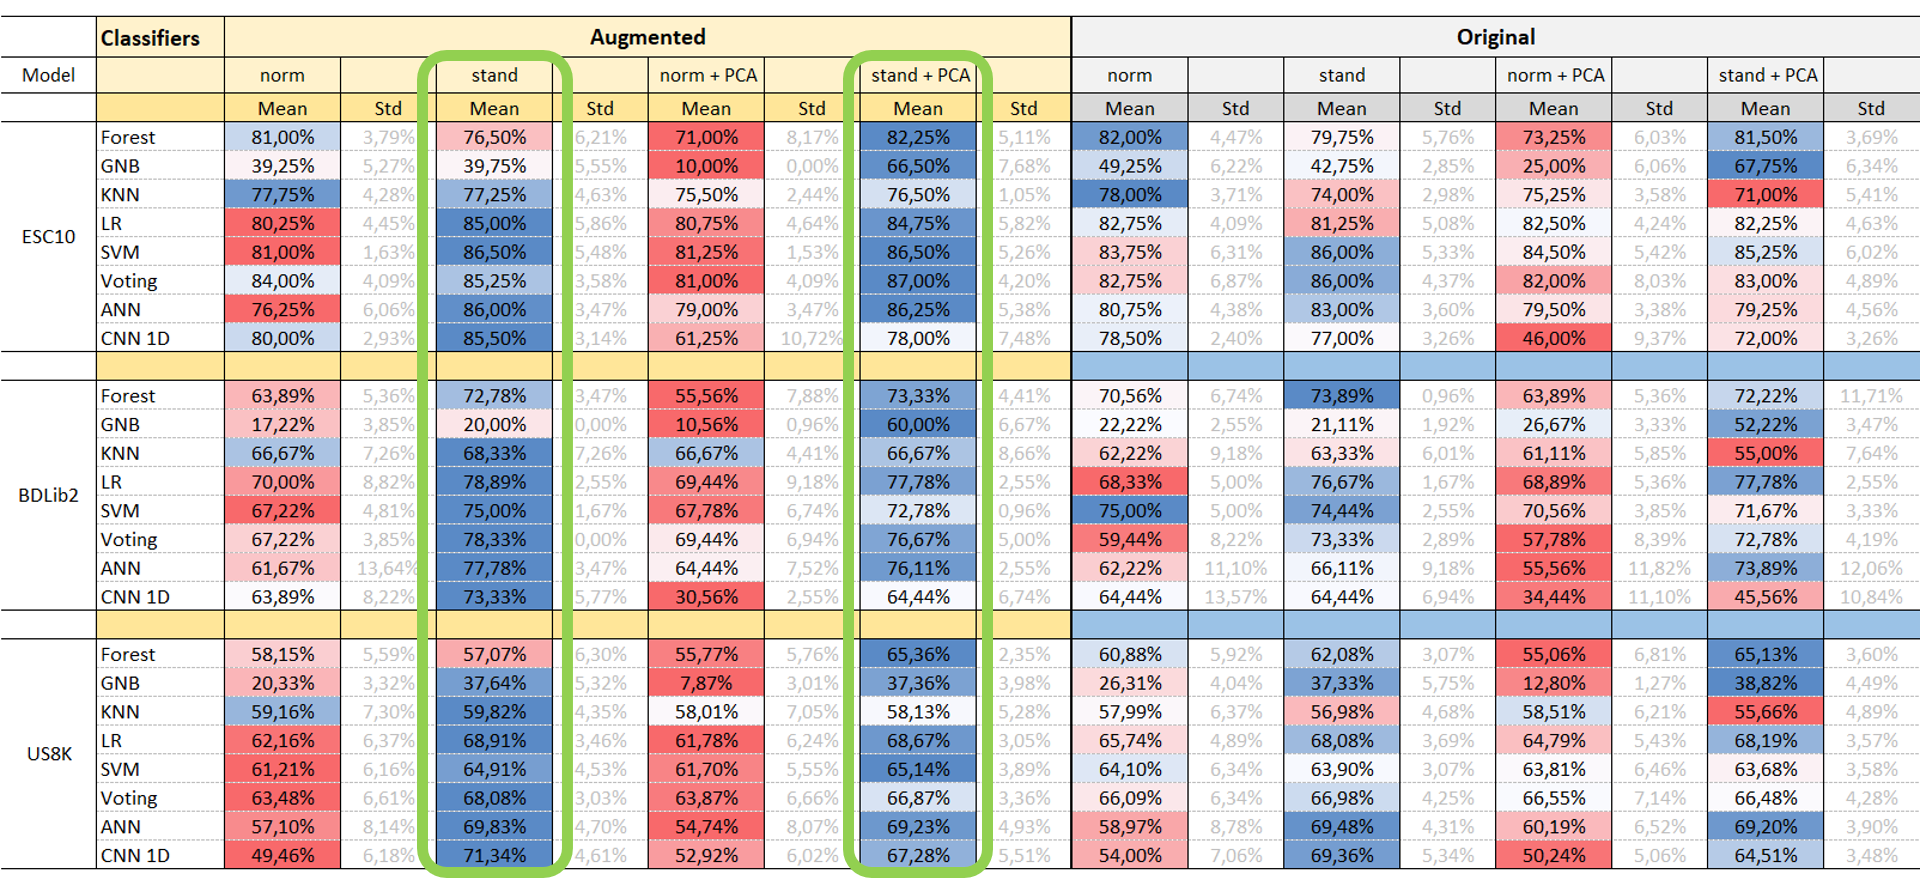
\includegraphics[width=1\textwidth]{resources/images/060-results/Results_classification_overview_aug_x_ori_1.png}
    \smallcaption{Source: Author}
\end{table}

When analyzing the entire datasets with their respective classifiers, notable performance was observed among classical machine learning techniques, with \textbf{\gls{lr}} and \textbf{\gls{svm}} emerging as the top-performers. Among ensemble methods, \textbf{Voting soft} proved effective, while in the realm of neural networks, both \textbf{\gls{ann}} and \textbf{\gls{cnn} 1D} demonstrated strong performance, albeit with some variability across datasets. Consistently, a pattern emerged wherein models \textbf{augmented standardized} and \textbf{augmented standardized + \gls{pca}} yielded the best results, as illustrated dataset by dataset with color gradient in Table \ref{table:results_accuracy_overview_classifiers_aug_ori_2}. 

\begin{table}[ht!]
    \caption[Accuracy rates overview using the benchmark datasets - Models augmented x original (Focus on the classifiers dataset by dataset)]{Accuracy rates overview using the benchmark datasets - The color gradient is focused on the classifiers utilized in the models augmented and original, dataset by dataset.}
    \label{table:results_accuracy_overview_classifiers_aug_ori_2}
     \raggedright
    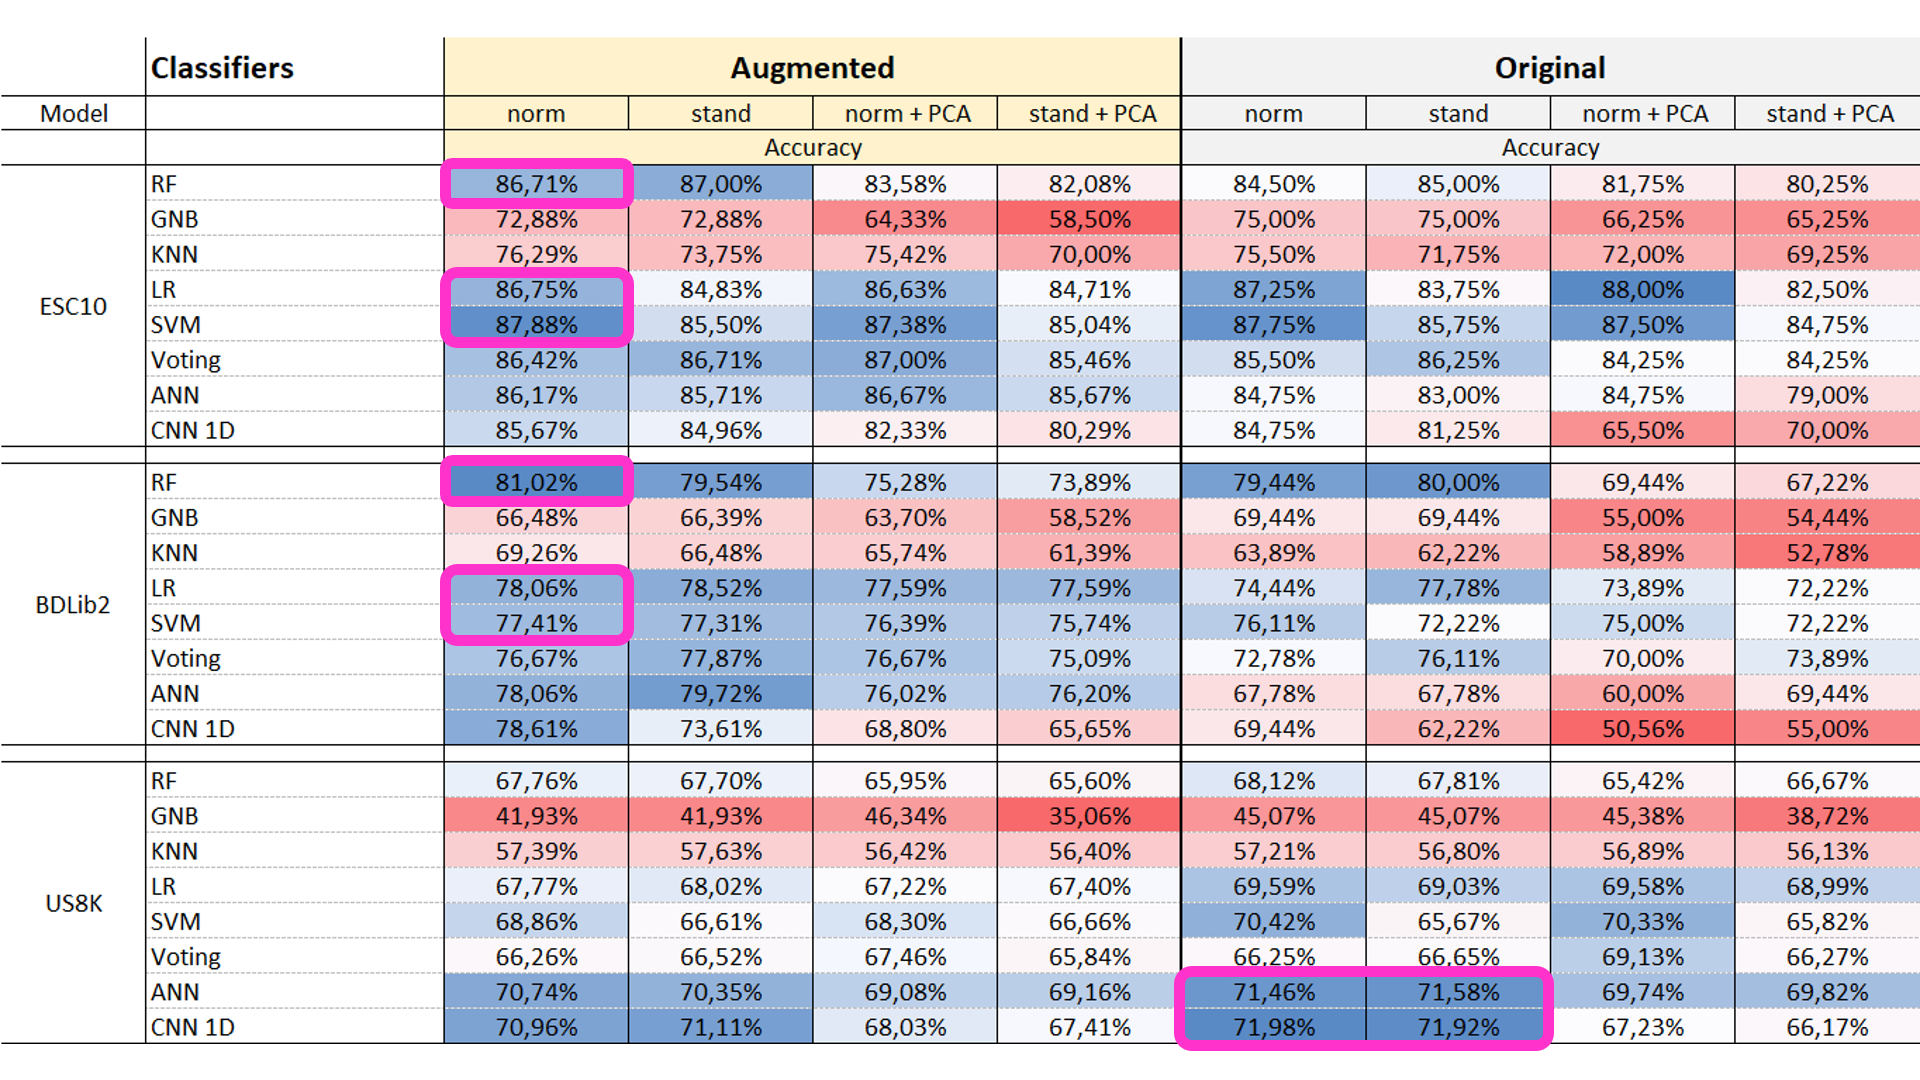
\includegraphics[width=1\textwidth]{resources/images/060-results/Results_classification_overview_aug_x_ori_2.png}
    \smallcaption{Source: Author}
\end{table}

The feature extraction process was evaluated following two methods: the first employed a sliding window of 1 \gls{s}, sampling rate of 22.050 \gls{hz} and 50\% overlapping, while the second method utilized entire audio file as input also with sampling rate of 22.050 \gls{hz}. For the top-performing classifiers using the original audio data, the accuracy rates increased on average 2,0\% in the ESC-10, 13,8\% in the BDLib2, and 0,7\% in the \gls{us8k}. On the other hand, when using the augmented datasets, the accuracy rates decreased on average 2,7\% in the ESC-10, 1,8\% in the BDLib2, and 1,0\% in the \gls{us8k}. The slight decrease in accuracy rates noticeable with the windowed method is barely evident from the gradient colors of the top-performing classifiers showcased in Table \ref{table:results_accuracy_overview_features_windowed}.


%To confirm these two models, it's planned to evaluate the Jaccard coefficient using bootstrap sampling according to \cite {Ho2020}.


\begin{table}[ht!]
    \caption[Accuracy rates overview using the benchmark datasets - Models augmented x windowed (Focus on the classifiers dataset by dataset)]{Accuracy rates overview using the benchmark datasets - The color gradient is focused on the classifiers utilized in the models augmented and windowed, dataset by dataset.}
    \label{table:results_accuracy_overview_features_windowed}
     \raggedright
    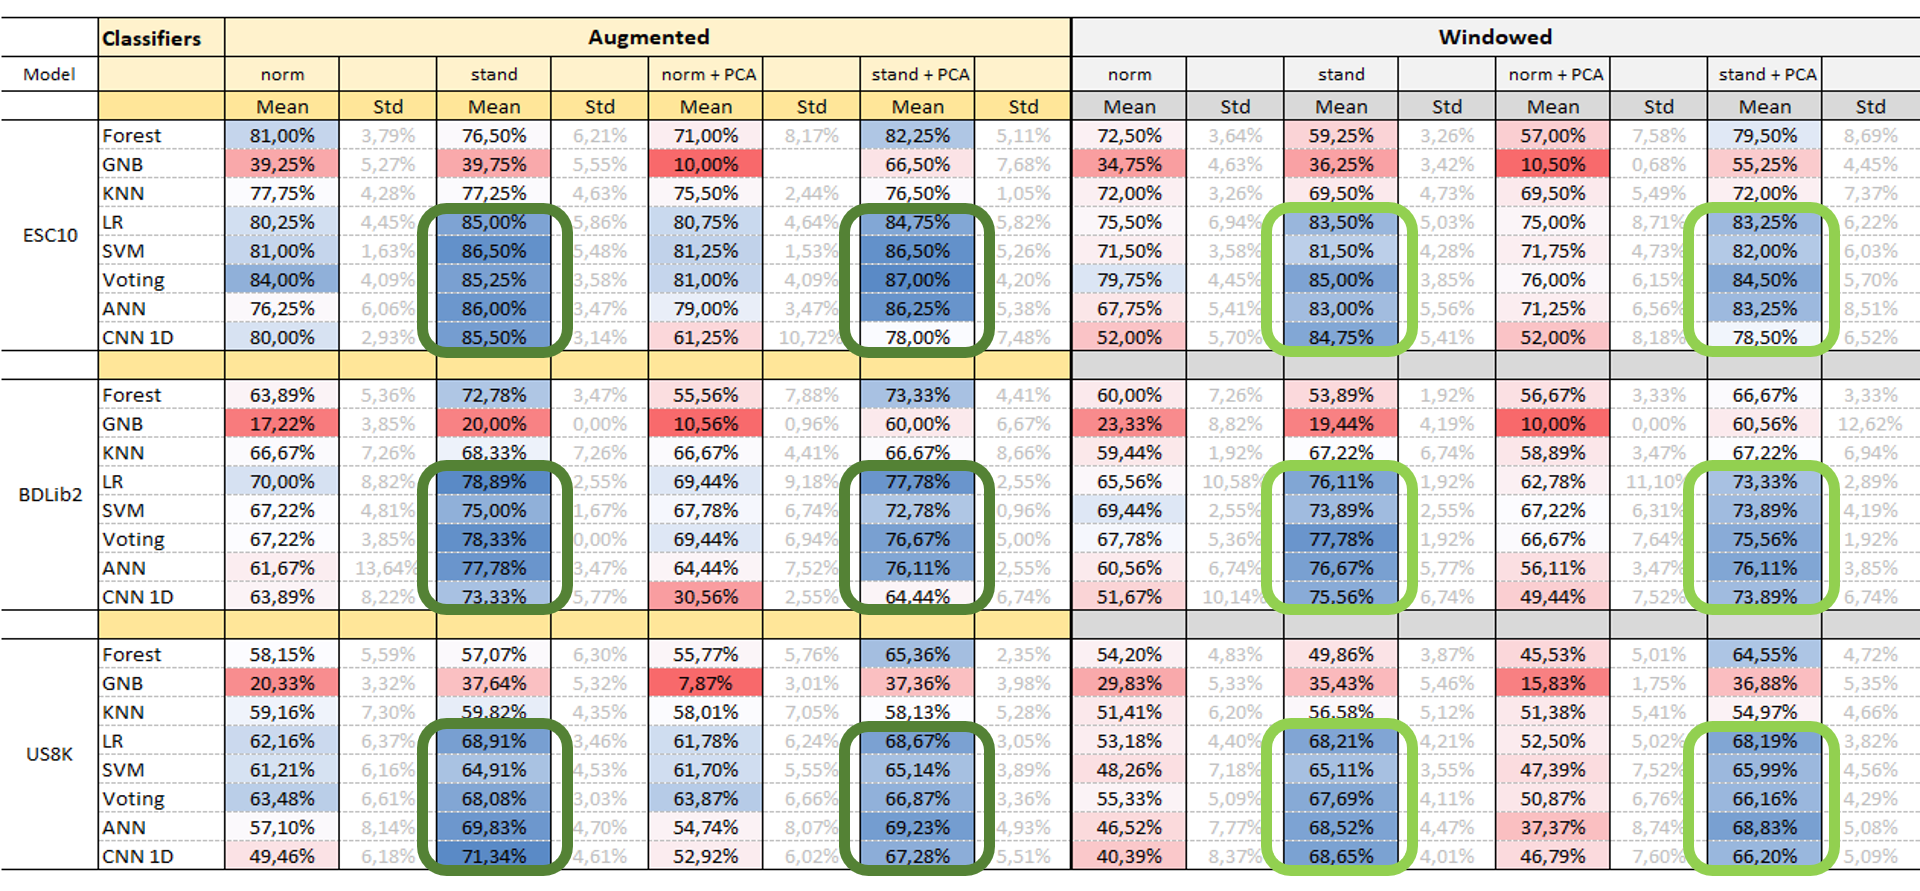
\includegraphics[width=1\textwidth]{resources/images/060-results/Results_classification_overview_aug_x_ori_3.png}
    \smallcaption{Source: Author}
\end{table}

Thus far, the results have shown that the utilization of \gls{pca} had minimal impact on the classifiers, with the exception of the \gls{cnn} 1D. While the sliding window method did decrease the accuracy rates of the top-performers, the reduction was mild, and the advantage to have an audio signal recognized in such a short term outweighs this reduction. Overall, it is important to note that neither the \gls{cnn} 2D nor other metrics, such as memory allocation, processing memory, and response time, were assessed. Therefore, while these initial findings are promising, it is premature to definitively conclude that this approach (\gls{pca}) is heading in the correct direction.

To finish the feature selection evaluation, a few investigations were also performed using mutual information from \index{scikit-learn}scikit-learn. Mutual information is calculated between two variables and measures the reduction in uncertainty for one variable given a known value of the other variable. Given two random variables $X$ and $Y$, it can be stated formally as follows:

\begin{equation}
    \label{eq:results_} 
    I(X ; Y) = H(X) - H(X | Y) \quad \text{With entropy:} \quad H = - \sum_i^C p_i \log_2p_i
\end{equation}

Where $I(X ; Y)$ is the mutual information for $X$ and $Y$, $H(X)$ is the entropy for $X$, $H(X | Y)$ is the conditional entropy for $X$ given $Y$, and $p_i$ is the probability of randomly picking an element of class $i$ (i.e. the proportion of the dataset made up of class $i$). Since mutual information is a measure of dependence or “mutual dependence” between two random variables, the result measure is symmetrical, meaning that $I(X ; Y) = I(Y ; X)$, measured as units of bits.

To establish a logical parameter, a threshold was calculated by taking the mean of the mutual information, considering only the features surpassing this threshold. Figure \ref{fig:results_mutual_information} illustrates an example using the ESC-10 dataset, displaying 375 features in the upper image and 207 in the lower image after applying the $KBest$ feature selection based on mutual information. Remarkably, none of the native 12 features from Table \ref{table:features_array_composition} were completely discarded, and among the statistics features - mean, median, std, skewness and kurtosis - the latter two were the least frequently selected. It is noteworthy that the number of selected features is directly influenced by the dataset and the information within the k-fold. Following cross-validation, the number of features selected averaged 202 $\pm$ 7 for ESC-10, 168 $\pm$ 18 for BDLib2, 178 $\pm$ 3 for \gls{us8k}, and 168 $\pm$ 5 for the tailored dataset US8k\_AV.

\begin{figure}[htbp]
    \raggedright
        \caption{Original features x selected features using mutual information with threshold established above the mean of the mutual information.}
        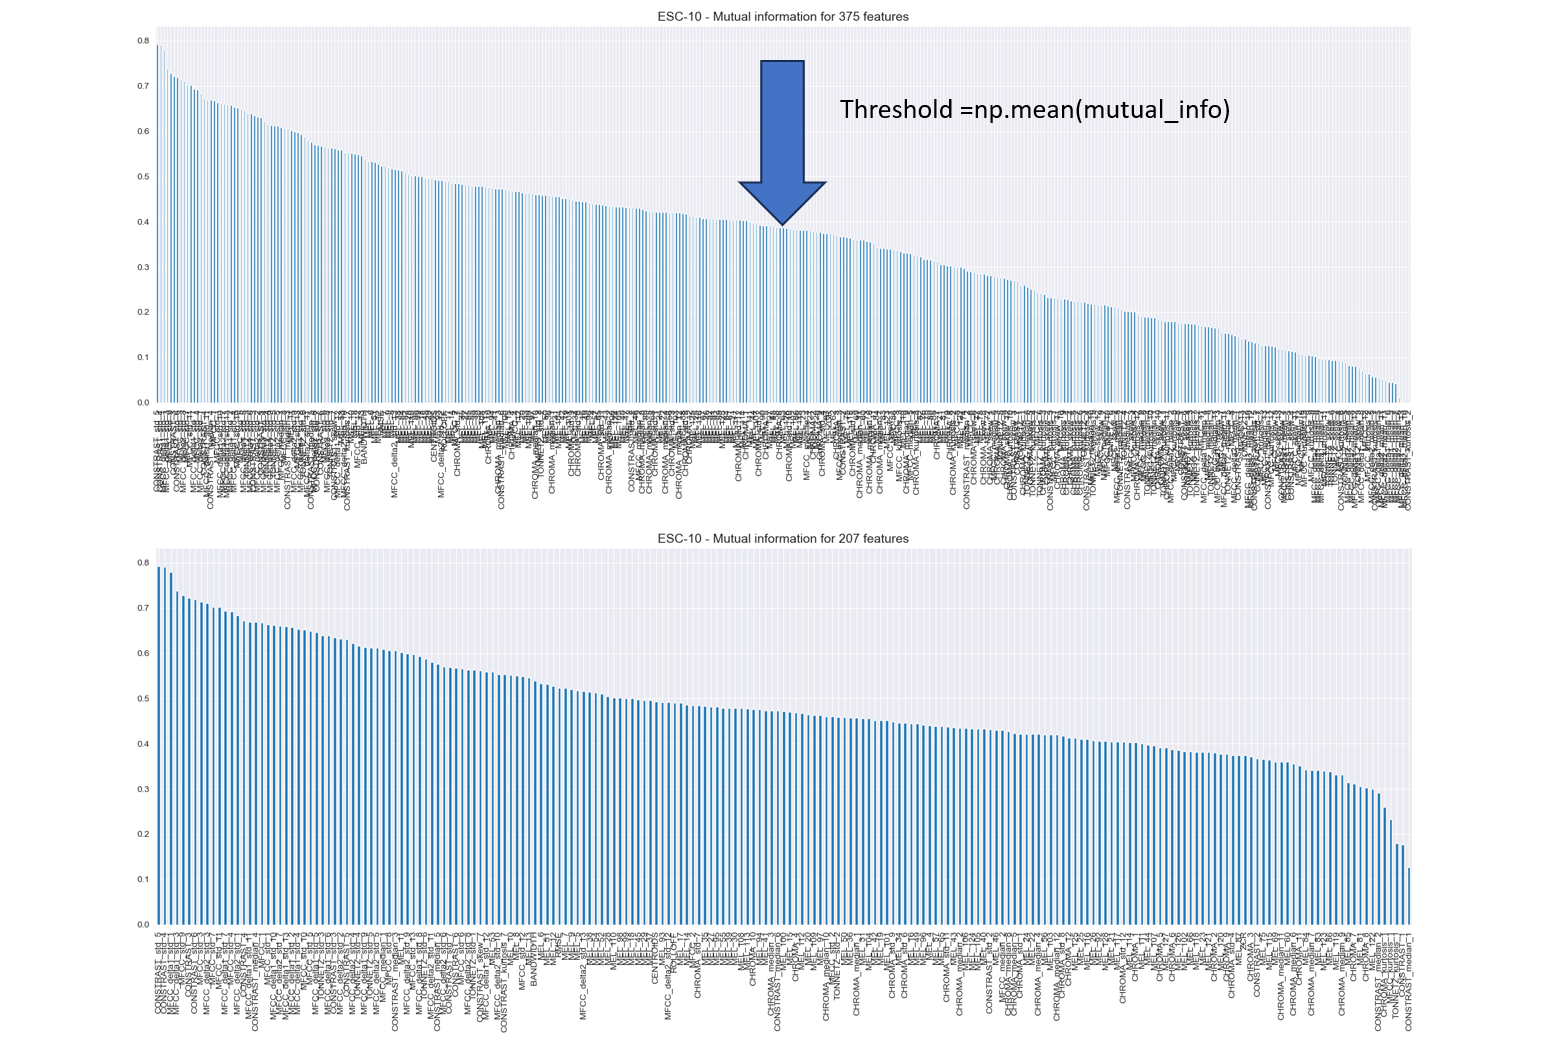
\includegraphics[width=1\textwidth]{resources/images/060-results/Results_classification_mutual_information_1.png}
        \smallcaption{Source: Author}
        \label{fig:results_mutual_information}
\end{figure}

The Random Forest and \gls{gnb} classifiers performed better when mutual information was utilized. Conversely, the accuracy rates of the remaining classifiers significantly worsened and no conclusion could be drawn on \gls{svm} because the algorithm didn't converge in the \gls{us8k} dataset, however, \gls{svm} will most likely worsen too given that it worsened in the ESC-10 and BDLib2 datasets where it converged. Notably, Random Forest matched the top-performing classifiers in the  US8K\_AV dataset and therefore, it continues as a strong candidate to be further evaluated considering other metrics such as processing memory, allocation memory and response time. Figure \ref{fig:results_mutual_information_boxplot} illustrates the accuracy results of the datasets using box plots for the augmented non-windowed model, highlighting the improvements (in green) against the highest accuracy results among the classifiers and models.

\begin{figure}[htbp]
    \raggedright
        \caption{Box plot of the accuracy results after utilizing mutual information in the augmented non-windowed models.}
        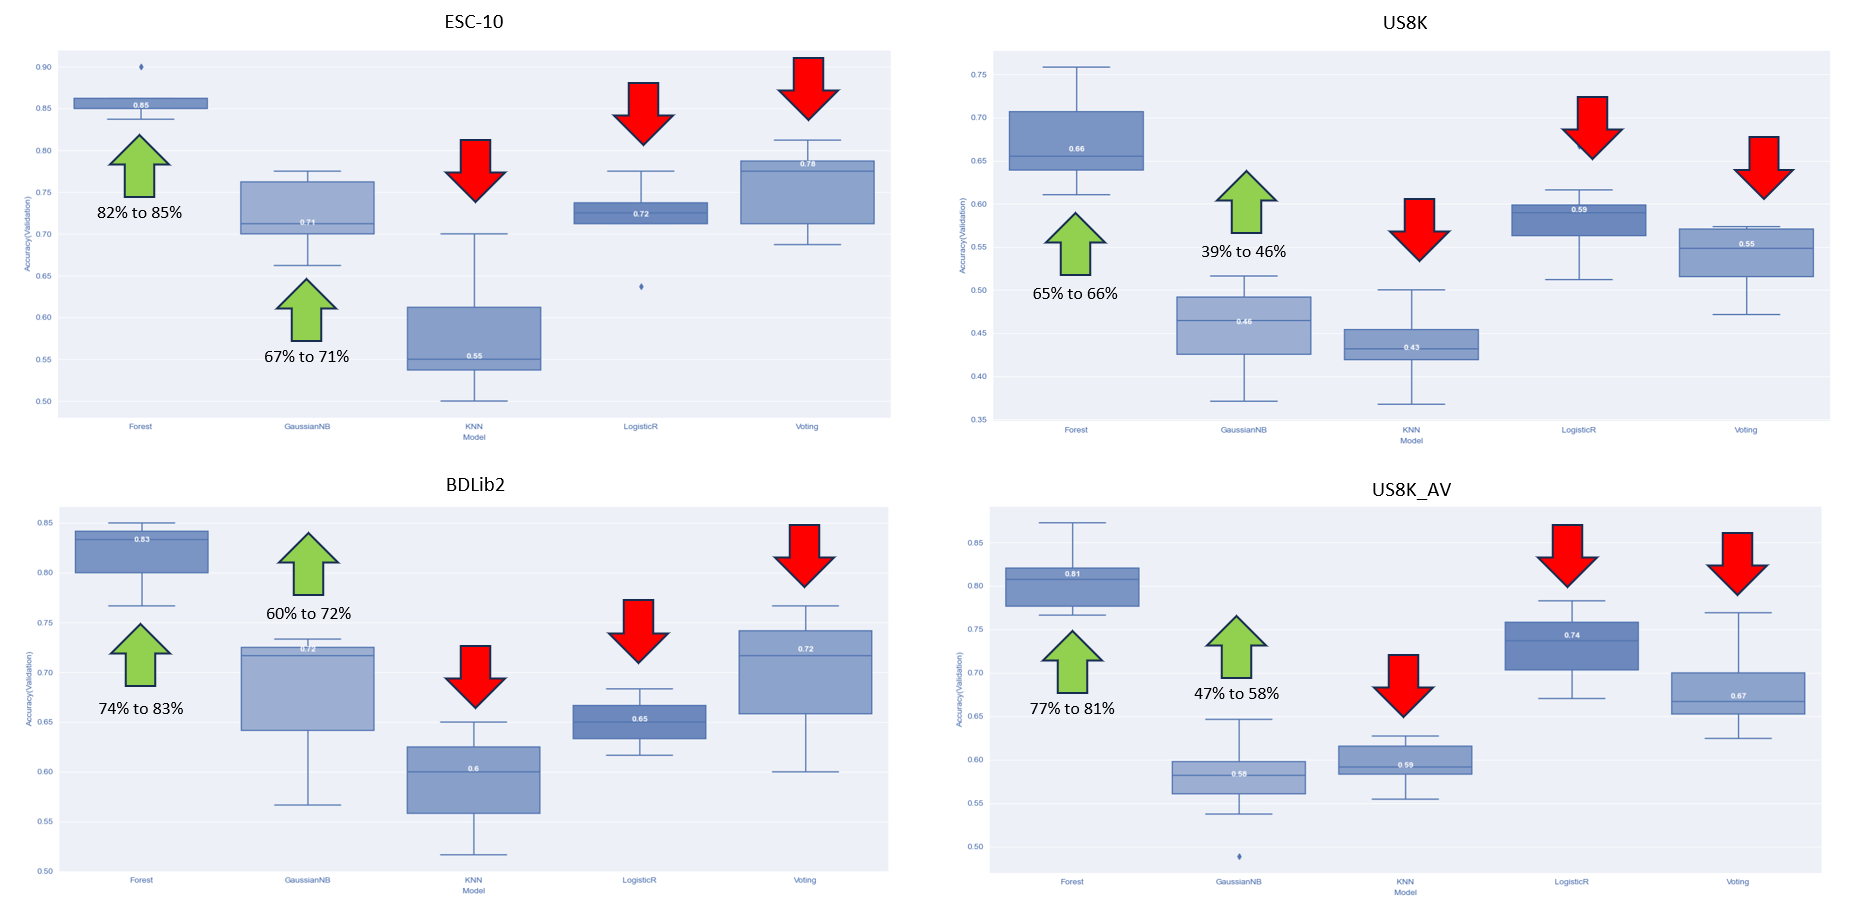
\includegraphics[width=1\textwidth]{resources/images/060-results/Results_classification_mutual_information_2.png}
        \smallcaption{Source: Author}
        \label{fig:results_mutual_information_boxplot}
\end{figure}

% Specific objective b).

The dataset created in subsection \ref{subsec:dataset_US8K-AV}, referred to as US8K\_AV, consists of 4.358 files distributed across 5 classes. These files collectively represent a total duration of 4,84 hours of recorded sounds. To maintain consistency and facilitate accuracy comparisons, the original 10-fold split for cross-validation from the source dataset (\gls{us8k}) was retained.

Similarly to the \gls{us8k} dataset, the augmentation process also resulted in a slight improvement (1,1\%) in accuracy rates for the top-performing classifiers. However, there were no significant differences observed when comparing the overall results within this dataset with those obtained using other datasets. Notably, the machine learning technique \textbf{\gls{lr}} consistently outperformed other methods with averaged accuracy of 81\%, while among the neural networks, \textbf{\gls{cnn} 1D} emerged as the most effective model with 82\% on the standardized models, dropping to 79\% when \gls{pca} is utilized. Table \ref{table:results_accuracy_overview_us8k_av_aug_ori_1} depicts the accuracy rates of the US8K\_AV together with the confusion matrices for the best results, and although not explicitly illustrated in the table, the recall on the \gls{ann} model was more estable (82,10\% $\pm$ 0,65\%) than the \gls{cnn} 1D model (80,64\% $\pm$ 3,00\%).  Similarly to the findings presented in Table \ref{table:results_accuracy_overview_features_windowed}, the accuracy results of the most effective classifiers on the US8K\_AV dataset exhibited a marginal decline of 1\% when employing the sliding process. This reduction was once again scarcely perceptible, as illustrated by the color gradient showcased in Table \ref{table:results_accuracy_overview_us8k_av_aug_wind_1}.

\begin{table}[ht!]
    \caption[Accuracy rates overview and confusion matrices using the tailored dataset US8K\_AV - Models augmented x original (Focus on the classifiers dataset by dataset)]{Accuracy rates overview and confusion matrices of the best models using the tailored dataset US8K\_AV - The color gradient is focused on the classifiers utilized in the models augmented and original, dataset by dataset.}
    \label{table:results_accuracy_overview_us8k_av_aug_ori_1}
     \raggedright
    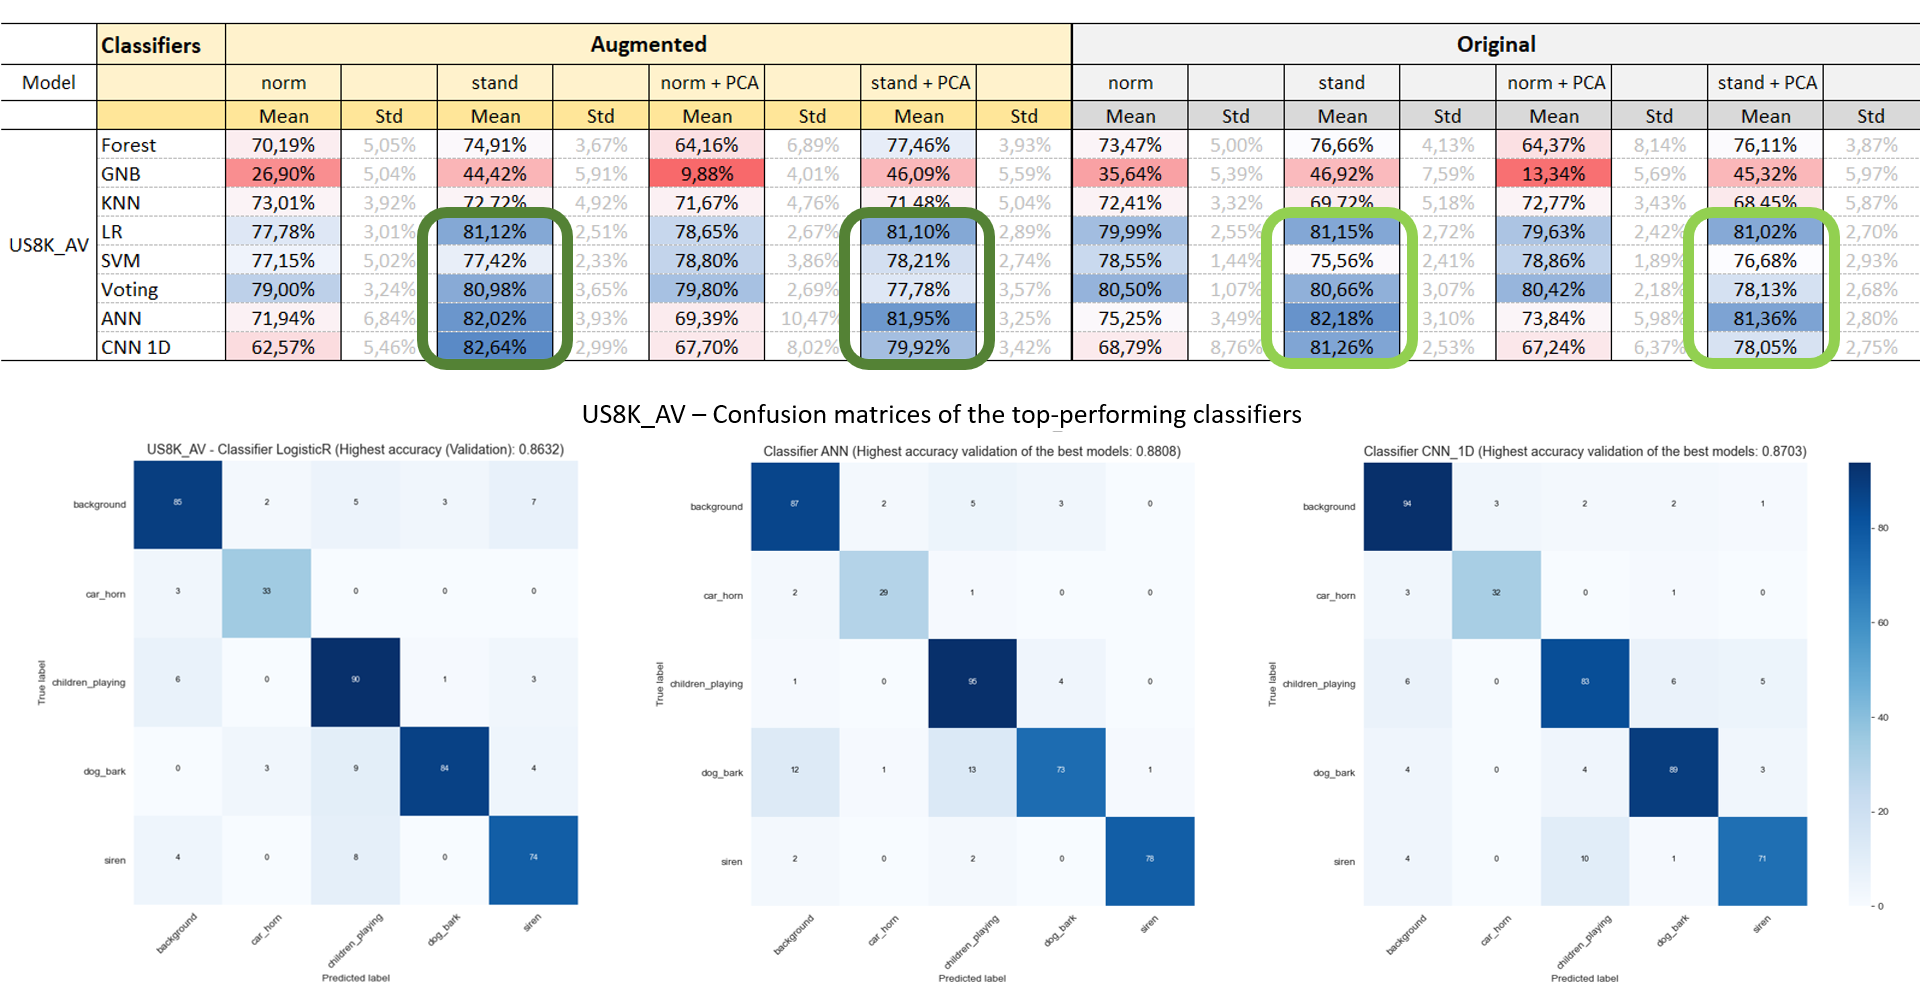
\includegraphics[width=1\textwidth]{resources/images/060-results/Results_classification_overview_us8k_av_aug_x_ori_1.png}
    \smallcaption{Source: Author}
\end{table}

\begin{table}[ht!]
    \caption[Accuracy rates overview using using the tailored dataset US8K\_AV - Models augmented x windowed (Focus on the classifiers dataset by dataset)]{Accuracy rates overview using the tailored dataset US8K\_AV - The color gradient is focused on the classifiers utilized in the models augmented and windowed, dataset by dataset.}
    \label{table:results_accuracy_overview_us8k_av_aug_wind_1}
     \raggedright
    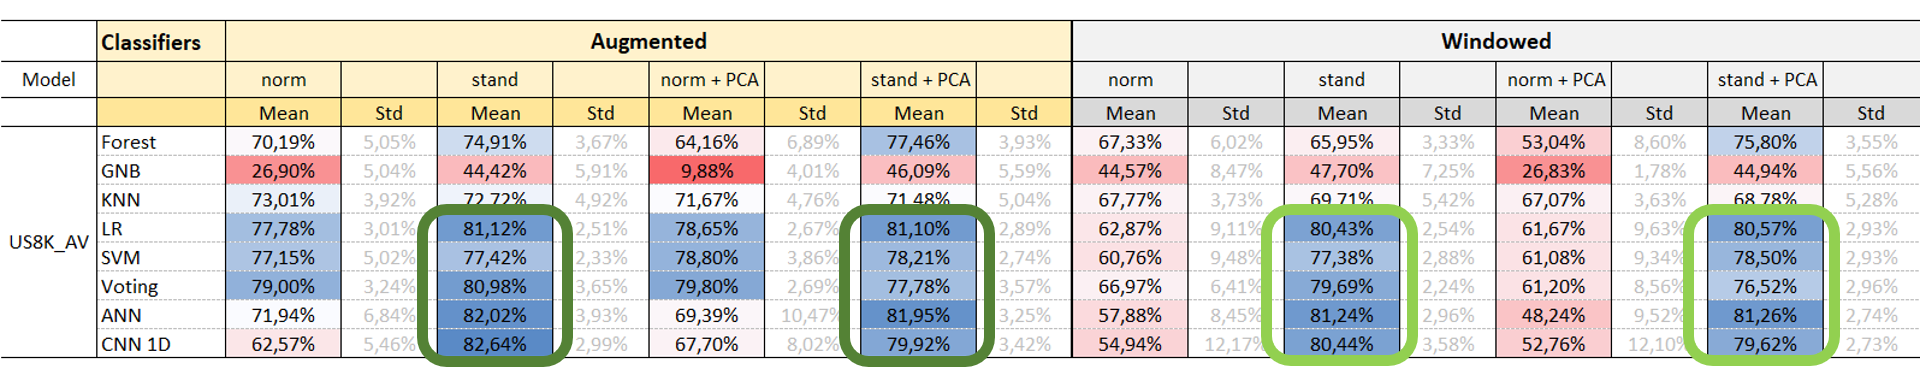
\includegraphics[width=1\textwidth]{resources/images/060-results/Results_classification_overview_us8k_av_aug_x_ori_2.png}
    \smallcaption{Source: Author}
\end{table}

Now that benchmark and tailored datasets are defined, the next step is to implement a \gls{cnn} 2D model utilizing aggregated features (log-mel spectrogram, Tonnetz, \gls{sct} and Chroma), compare it with a model that tries to capture the sound variation along time (log-mel spectrogram, $\triangle$\gls{mfcc} and $\triangle\triangle$\gls{mfcc}), and assess the remaining evaluation metrics (processing memory, allocation memory and response time). In the evaluation flow, deploy the wining classifier on the RaspBerry Pi and finish by assessing the benchmark metrics from the training and classification flow.


